% ============================================================
% 初升高衔接讲义 — 因式分解与整式运算强化
% 编译命令：xelatex -interaction=nonstopmode 衔接2_因式分解与整式运算强化.tex
% ============================================================
\documentclass[12pt, a4paper]{ctexart}
\usepackage[margin=2.2cm]{geometry}
\usepackage{amsmath, amssymb}
\usepackage{enumitem}
\usepackage{tcolorbox}
\usepackage{booktabs}
\usepackage{array}
\usepackage{fancyhdr}
\usepackage{xcolor}
\usepackage{tikz}
\usepackage{hyperref}
\usepackage{graphicx}
\usepackage{multirow}
\usepackage{textcomp}
\usepackage{pgfplots}
\pgfplotsset{compat=1.18}

% 颜色定义
\definecolor{mainblue}{RGB}{41, 98, 168}
\definecolor{lightblue}{RGB}{230, 240, 255}
\definecolor{tipgreen}{RGB}{34, 139, 87}
\definecolor{lightgreen}{RGB}{235, 250, 240}
\definecolor{warnred}{RGB}{200, 50, 50}
\definecolor{lightred}{RGB}{255, 240, 240}
\definecolor{examorange}{RGB}{210, 120, 20}
\definecolor{lightorange}{RGB}{255, 248, 235}
\definecolor{apppurple}{RGB}{120, 60, 170}
\definecolor{lightpurple}{RGB}{245, 238, 255}

% 页眉页脚
\pagestyle{fancy}
\fancyhf{}
\fancyhead[L]{\small\textcolor{mainblue}{\textbf{初升高衔接 · 因式分解与整式运算}}}
\fancyhead[R]{\small\textcolor{mainblue}{衔接讲义（二）}}
\fancyfoot[C]{\small —\ \thepage\ —}
\renewcommand{\headrulewidth}{0.6pt}
\renewcommand{\headrule}{\hbox to\headwidth{\color{mainblue}\leaders\hrule height \headrulewidth\hfill}}
\renewcommand{\footrulewidth}{0pt}

% tcolorbox 样式
\newtcolorbox{knowledgebox}[1][]{%
  colback=lightblue, colframe=mainblue,
  fonttitle=\bfseries\large, title=#1,
  arc=3mm, boxrule=0.8pt,
  left=8pt, right=8pt, top=6pt, bottom=6pt
}

\newtcolorbox{tipbox}[1][]{%
  colback=lightgreen, colframe=tipgreen,
  fonttitle=\bfseries, title=#1,
  arc=2mm, boxrule=0.6pt,
  left=6pt, right=6pt, top=4pt, bottom=4pt
}

\newtcolorbox{warnbox}[1][]{%
  colback=lightred, colframe=warnred,
  fonttitle=\bfseries, title=#1,
  arc=2mm, boxrule=0.6pt,
  left=6pt, right=6pt, top=4pt, bottom=4pt
}

\newtcolorbox{examplebox}[1][]{%
  colback=lightorange, colframe=examorange,
  fonttitle=\bfseries, title=#1,
  arc=3mm, boxrule=0.8pt,
  left=8pt, right=8pt, top=6pt, bottom=6pt
}

\newtcolorbox{appbox}[1][]{%
  colback=lightpurple, colframe=apppurple,
  fonttitle=\bfseries, title=#1,
  arc=3mm, boxrule=0.8pt,
  left=8pt, right=8pt, top=6pt, bottom=6pt
}

\setCJKmainfont{Hiragino Sans GB}
\setCJKsansfont{Heiti SC}

\begin{document}

% ============ 标题页 ============
\begin{center}
{\Huge\bfseries\textcolor{mainblue}{初升高衔接（二）}}\\[12pt]
{\LARGE\textcolor{mainblue}{因式分解与整式运算强化}}\\[10pt]
\rule{0.6\textwidth}{1pt}\\[8pt]
{\normalsize 适用：准高一学生\quad |\quad 重点：十字相乘、配方、裂项}
\end{center}
\vspace{6pt}

% ==============================================================
% 第一部分：知识点讲解
% ==============================================================
\section*{\textcolor{mainblue}{一、知识点讲解}}

% ───────── 1.1 提公因式法 ─────────
\subsection*{1.1\quad 提公因式法}

\begin{knowledgebox}[什么是"因式分解"？]
把一个多项式化成几个整式的\textbf{积}的形式，叫做因式分解。\\[4pt]
\textbf{关键口诀：}左边是"和/差"，右边是"积"——和差化积！\\[4pt]
因式分解与整式乘法互为\textbf{逆运算}，例如：\\
整式乘法：$a(b+c)=ab+ac$；\quad 因式分解：$ab+ac=a(b+c)$。
\end{knowledgebox}

\begin{knowledgebox}[提公因式法——第一步永远先做这个！]
\textbf{步骤：}\\[3pt]
① 找各项系数的\textbf{最大公因数}；\\
② 找各项都含有的\textbf{相同字母}，取最低次幂；\\
③ 把公因式提到括号外面，括号内写除以公因式后的各项。\\[6pt]
\textbf{例：}\quad $6x^3y - 9x^2y^2 + 3x^2y$\\[3pt]
系数最大公因数：$\gcd(6,9,3)=3$；\\
字母公因式：$x^2y$（$x$ 取最低次 $2$，$y$ 取最低次 $1$）；\\
所以公因式 $= 3x^2y$。\\[3pt]
$6x^3y - 9x^2y^2 + 3x^2y = 3x^2y \cdot 2x - 3x^2y \cdot 3y + 3x^2y \cdot 1 = 3x^2y(2x - 3y + 1)$。
\end{knowledgebox}

\begin{warnbox}[易错提醒]
\begin{enumerate}[leftmargin=18pt]
\item 提完公因式后，括号里\textbf{每一项}都要除以公因式，不要漏项！
\item 公因式是"系数取最小、字母取最低次"，不是最大次。
\item 提取负号时，括号内各项要\textbf{全部变号}。
\end{enumerate}
\end{warnbox}

% ───────── 1.2 平方差公式 ─────────
\subsection*{1.2\quad 平方差公式}

\begin{knowledgebox}[平方差公式]
\[
\boxed{a^2 - b^2 = (a+b)(a-b)}
\]
\textbf{语言表述：}两个数的平方差，等于这两个数的和乘以这两个数的差。\\[6pt]
\textbf{使用条件（三个同时满足）：}\\
① 两项；\quad ② 都是平方形式；\quad ③ 中间是\textbf{减号}。\\[6pt]
\textbf{例：}\quad $4x^2 - 9y^2 = (2x)^2 - (3y)^2 = (2x+3y)(2x-3y)$。
\end{knowledgebox}

\begin{tipbox}[推广——多次使用平方差]
$a^4 - b^4 = (a^2+b^2)(a^2-b^2) = (a^2+b^2)(a+b)(a-b)$。\\[3pt]
遇到高次幂的差，可以反复"降次"使用平方差公式。
\end{tipbox}

% ───────── 1.3 完全平方公式 ─────────
\subsection*{1.3\quad 完全平方公式}

\begin{knowledgebox}[完全平方公式]
\[
\boxed{(a+b)^2 = a^2 + 2ab + b^2}
\]
\[
\boxed{(a-b)^2 = a^2 - 2ab + b^2}
\]
\textbf{语言表述：}两数和（差）的平方，等于它们的平方和，加（减）它们积的 2 倍。\\[6pt]
\textbf{识别口诀：}首平方 + 尾平方 + 2 倍乘积（注意符号！）。\\[6pt]
\textbf{例：}\quad $x^2 + 6x + 9 = x^2 + 2 \cdot x \cdot 3 + 3^2 = (x+3)^2$。
\end{knowledgebox}

\begin{warnbox}[易错提醒]
\begin{enumerate}[leftmargin=18pt]
\item $(a+b)^2 \neq a^2+b^2$，\textbf{中间的 $2ab$ 千万不能丢}！这是最常见的错误。
\item 判断是否为完全平方式：看首尾两项是否都是平方，中间项是否恰好是"2 倍乘积"。
\item 中间项的\textbf{符号}要与一次项的符号一致。
\end{enumerate}
\end{warnbox}

% ───────── 1.4 十字相乘法 ─────────
\subsection*{1.4\quad 十字相乘法（重点！高中大量使用）}

\begin{knowledgebox}[十字相乘法——二次三项式的分解]
对于 $x^2 + (p+q)x + pq$ 型的二次三项式，可以分解为：
\[
\boxed{x^2 + (p+q)x + pq = (x+p)(x+q)}
\]
\textbf{核心思想：}找两个数 $p$ 和 $q$，使得：\\
\begin{center}
$p \times q$ = 常数项（末项），\quad $p + q$ = 一次项系数。
\end{center}
\vspace{4pt}
\textbf{十字相乘图示：}\\[6pt]
\begin{center}
\begin{tikzpicture}[scale=1.0]
% 左列
\node at (0, 0.5) {$x$};
\node at (0, -0.5) {$x$};
% 右列
\node at (2, 0.5) {$p$};
\node at (2, -0.5) {$q$};
% 十字交叉线
\draw[thick, mainblue] (0.3, 0.5) -- (1.7, -0.5);
\draw[thick, mainblue] (0.3, -0.5) -- (1.7, 0.5);
% 结果标注
\node[right, mainblue] at (2.8, 0.5) {\small 交叉相乘之和 $= p+q$（一次项系数）};
\node[right, mainblue] at (2.8, -0.5) {\small 同行相乘：$x \cdot x = x^2$，$p \cdot q = pq$};
\end{tikzpicture}
\end{center}
\vspace{4pt}
\textbf{例：}\quad 分解 $x^2 + 5x + 6$。\\
找 $p, q$ 使得 $p+q=5$，$pq=6$。\\
尝试：$p=2, q=3$ \checkmark\quad（$2+3=5$，$2\times3=6$）\\
所以 $x^2+5x+6=(x+2)(x+3)$。
\end{knowledgebox}

\begin{knowledgebox}[系数不为 1 的十字相乘：$ax^2+bx+c$ 型]
当二次项系数 $a \neq 1$ 时，需要用"双十字"法：\\[4pt]
把 $a$ 拆成两个因数 $a_1 \cdot a_2$，把 $c$ 拆成两个因数 $c_1 \cdot c_2$，\\
使得十字交叉相乘之和等于 $b$：$a_1 c_2 + a_2 c_1 = b$。\\[6pt]
\begin{center}
\begin{tikzpicture}[scale=1.0]
\node at (0, 0.5) {$a_1 x$};
\node at (0, -0.5) {$a_2 x$};
\node at (2.5, 0.5) {$c_1$};
\node at (2.5, -0.5) {$c_2$};
\draw[thick, mainblue] (0.6, 0.5) -- (2.1, -0.5);
\draw[thick, mainblue] (0.6, -0.5) -- (2.1, 0.5);
\node[right, mainblue, font=\small] at (3.2, 0.5) {$a_1 c_2 + a_2 c_1 = b$};
\node[right, mainblue, font=\small] at (3.2, -0.5) {则 $ax^2+bx+c=(a_1 x + c_1)(a_2 x + c_2)$};
\end{tikzpicture}
\end{center}
\vspace{4pt}
\textbf{例：}\quad 分解 $2x^2+7x+3$。\\
$a=2=2\times1$，$c=3=3\times1$（或 $1\times3$，或 $(-1)\times(-3)$ 等）。\\[3pt]
\begin{center}
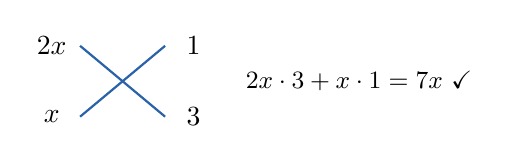
\begin{tikzpicture}[scale=0.9]
\node at (0, 0.5) {$2x$};
\node at (0, -0.5) {$x$};
\node at (2, 0.5) {$1$};
\node at (2, -0.5) {$3$};
\draw[thick, mainblue] (0.4, 0.5) -- (1.6, -0.5);
\draw[thick, mainblue] (0.4, -0.5) -- (1.6, 0.5);
\node[right, font=\small] at (2.6, 0) {$2x \cdot 3 + x \cdot 1 = 7x$ \checkmark};
\end{tikzpicture}
\end{center}
所以 $2x^2+7x+3=(2x+1)(x+3)$。
\end{knowledgebox}

\begin{tipbox}[十字相乘的训练技巧]
\begin{enumerate}[leftmargin=18pt]
\item 先处理符号：常数项为正则 $p, q$ 同号（看一次项系数定正负）；常数项为负则 $p, q$ 异号。
\item 先列常数项的因数对，再逐个检验和是否等于一次项系数。
\item 常见因数分解要熟：$6=1\times6=2\times3$，$12=1\times12=2\times6=3\times4$，等等。
\item 分解完毕后，\textbf{用展开验证}！养成检查的习惯。
\end{enumerate}
\end{tipbox}

% ───────── 1.5 分组分解法 ─────────
\subsection*{1.5\quad 分组分解法}

\begin{knowledgebox}[分组分解法]
当多项式有四项（或更多）且无法直接提公因式时，可以\textbf{分组}后再分别提公因式。\\[6pt]
\textbf{步骤：}\\
① 把多项式分成两组（通常每组两项）；\\
② 分别对每组提公因式；\\
③ 若两组提出后有\textbf{相同的因式}，再整体提出。\\[6pt]
\textbf{例：}\quad $ax + ay + bx + by$\\
$= a(x+y) + b(x+y)$\quad（分组，分别提公因式）\\
$= (x+y)(a+b)$\quad（再提公因式 $x+y$）。
\end{knowledgebox}

\begin{warnbox}[分组的关键]
分组方式\textbf{不是唯一的}，但必须保证分组后能继续分解。\\
如果分组后无法继续，说明分组方式不对，需要换一种分法试试。
\end{warnbox}

% ───────── 1.6 拆项添项法 ─────────
\subsection*{1.6\quad 拆项添项法（拓展）}

\begin{knowledgebox}[拆项添项法]
有时候多项式直接分组不行，需要\textbf{拆开}某一项或\textbf{添加再减去}某一项，创造分组分解的条件。\\[6pt]
\textbf{例：}\quad 分解 $x^3 + 3x^2 - 4$。\\[3pt]
观察到常数项 $-4$，可以拆成 $-1$ 和 $-3$（或 $+1$ 和 $-4$ 等）。\\
尝试：把 $3x^2$ 拆成 $4x^2 - x^2$：\\[3pt]
$x^3 + 3x^2 - 4 = x^3 - x^2 + 4x^2 - 4$\\
$= x^2(x-1) + 4(x^2-1)$\\
$= x^2(x-1) + 4(x+1)(x-1)$\\
$= (x-1)\big[x^2 + 4(x+1)\big]$\\
$= (x-1)(x^2 + 4x + 4)$\\
$= (x-1)(x+2)^2$。
\end{knowledgebox}

\begin{tipbox}[什么时候用拆项添项？]
\begin{enumerate}[leftmargin=18pt]
\item 高次多项式（三次及以上）无法直接分组时。
\item 常见策略：拆中间项（把高次项或低次项拆成两项之和/差）。
\item 也可以尝试"添一项再减同一项"，比如 $x^4+4 = x^4+4x^2+4-4x^2 = (x^2+2)^2-(2x)^2$。
\end{enumerate}
\end{tipbox}

% ───────── 1.7 整式运算 ─────────
\subsection*{1.7\quad 整式运算：幂运算与乘法公式}

\begin{knowledgebox}[幂运算法则]
\begin{enumerate}[leftmargin=18pt]
\item \textbf{同底数幂相乘：}\quad $a^m \cdot a^n = a^{m+n}$
\item \textbf{同底数幂相除：}\quad $a^m \div a^n = a^{m-n}$\quad（$a \neq 0$）
\item \textbf{幂的乘方：}\quad $(a^m)^n = a^{mn}$
\item \textbf{积的乘方：}\quad $(ab)^n = a^n b^n$
\item \textbf{零指数：}\quad $a^0 = 1$\quad（$a \neq 0$）
\item \textbf{负整数指数：}\quad $a^{-n} = \dfrac{1}{a^n}$\quad（$a \neq 0$）
\end{enumerate}
\end{knowledgebox}

\begin{knowledgebox}[常用乘法公式汇总]
\begin{enumerate}[leftmargin=18pt]
\item \textbf{平方差：}\quad $(a+b)(a-b) = a^2 - b^2$
\item \textbf{完全平方：}\quad $(a \pm b)^2 = a^2 \pm 2ab + b^2$
\item \textbf{立方和：}\quad $a^3 + b^3 = (a+b)(a^2 - ab + b^2)$
\item \textbf{立方差：}\quad $a^3 - b^3 = (a-b)(a^2 + ab + b^2)$
\item \textbf{完全立方：}\quad $(a \pm b)^3 = a^3 \pm 3a^2b + 3ab^2 \pm b^3$
\end{enumerate}
\end{knowledgebox}

% ───────── 1.8 整式除法 ─────────
\subsection*{1.8\quad 整式除法（多项式除以多项式）}

\begin{knowledgebox}[多项式除法——类比多位数除法]
\textbf{例：}\quad 计算 $(2x^3 + 3x^2 - 5x + 1) \div (x + 2)$。\\[6pt]
用长除法（类比竖式除法）：\\[3pt]
\begin{enumerate}[leftmargin=18pt]
\item $2x^3 \div x = 2x^2$，写在商的位置；\quad $2x^2 \cdot (x+2) = 2x^3 + 4x^2$；
\item 相减：$(2x^3+3x^2) - (2x^3+4x^2) = -x^2$；落下 $-5x$，得 $-x^2-5x$；
\item $-x^2 \div x = -x$；\quad $(-x)(x+2) = -x^2-2x$；
\item 相减：$(-x^2-5x)-(-x^2-2x) = -3x$；落下 $+1$，得 $-3x+1$；
\item $-3x \div x = -3$；\quad $(-3)(x+2) = -3x-6$；
\item 相减：$(-3x+1)-(-3x-6) = 7$（余数）。
\end{enumerate}
结果：$2x^2 - x - 3 \cdots\cdots 余\, 7$，即 $2x^3+3x^2-5x+1 = (x+2)(2x^2-x-3) + 7$。
\end{knowledgebox}

% ───────── 1.9 分式运算回顾 ─────────
\subsection*{1.9\quad 分式运算回顾}

\begin{knowledgebox}[分式的基本性质与运算]
\textbf{基本性质：}\quad $\dfrac{a}{b} = \dfrac{a \times c}{b \times c} = \dfrac{a \div c}{b \div c}$\quad（$b \neq 0, c \neq 0$）\\[8pt]
\textbf{加减法（通分）：}\quad $\dfrac{a}{b} \pm \dfrac{c}{d} = \dfrac{ad \pm bc}{bd}$\\[8pt]
\textbf{乘法：}\quad $\dfrac{a}{b} \cdot \dfrac{c}{d} = \dfrac{ac}{bd}$\\[8pt]
\textbf{除法：}\quad $\dfrac{a}{b} \div \dfrac{c}{d} = \dfrac{a}{b} \cdot \dfrac{d}{c} = \dfrac{ad}{bc}$\\[8pt]
\textbf{乘方：}\quad $\left(\dfrac{a}{b}\right)^n = \dfrac{a^n}{b^n}$
\end{knowledgebox}

\begin{warnbox}[分式运算注意事项]
\begin{enumerate}[leftmargin=18pt]
\item 分式运算的结果要化成\textbf{最简分式}（约分到不能再约为止）。
\item 分母不能为零——这是讨论分式问题时\textbf{首先要考虑}的条件。
\item 分式加减时，先通分再运算，不要"交叉相乘相加"。
\end{enumerate}
\end{warnbox}

% ───────── 1.10 高中常用技巧 ─────────
\subsection*{1.10\quad 高中常用技巧：配方、裂项、整体代换}

\begin{knowledgebox}[配方（配方法）]
把一个二次式变成"完全平方式 + 常数"的形式。\\[6pt]
\textbf{步骤：}\quad $ax^2+bx+c$\\[3pt]
① 提取 $a$：$= a\!\left(x^2 + \dfrac{b}{a}x\right) + c$；\\[3pt]
② 括号内配方：加减 $\left(\dfrac{b}{2a}\right)^2$；\\[3pt]
③ 整理：$= a\!\left(x + \dfrac{b}{2a}\right)^2 + c - \dfrac{b^2}{4a}$。\\[6pt]
\textbf{例：}\quad $x^2 + 6x + 5 = (x^2+6x+9) - 9 + 5 = (x+3)^2 - 4$。
\end{knowledgebox}

\begin{knowledgebox}[裂项（裂项相消法）]
把一个分式拆成两个（或多个）分式的差，使得求和时可以\textbf{逐项抵消}。\\[6pt]
\textbf{基本公式：}\quad $\dfrac{1}{n(n+1)} = \dfrac{1}{n} - \dfrac{1}{n+1}$\\[8pt]
\textbf{推广公式：}\quad $\dfrac{1}{n(n+k)} = \dfrac{1}{k}\!\left(\dfrac{1}{n} - \dfrac{1}{n+k}\right)$\\[8pt]
\textbf{例：}\quad $\displaystyle\sum_{k=1}^{n}\frac{1}{k(k+1)} = \sum_{k=1}^{n}\left(\frac{1}{k}-\frac{1}{k+1}\right) = 1 - \frac{1}{n+1} = \frac{n}{n+1}$。
\end{knowledgebox}

\begin{knowledgebox}[整体代换]
设 $t = $ 某个代数式，把问题转化为关于 $t$ 的问题。\\[6pt]
\textbf{例：}\quad 已知 $x + \dfrac{1}{x} = 3$，求 $x^2 + \dfrac{1}{x^2}$ 的值。\\[3pt]
设 $t = x + \dfrac{1}{x} = 3$，则 $t^2 = x^2 + 2 + \dfrac{1}{x^2}$，\\
所以 $x^2 + \dfrac{1}{x^2} = t^2 - 2 = 9 - 2 = 7$。
\end{knowledgebox}


% ==============================================================
% 第二部分：例题精讲
% ==============================================================
\section*{\textcolor{examorange}{二、例题精讲}}

% ──── 例题 1：基础因式分解 ────
\begin{examplebox}[【例题 1】基础因式分解——提公因式 + 公式]
因式分解：\\[3pt]
(1)\;$6x^3 - 24x$ \qquad (2)\;$3a^2b - 12ab^2 + 12b^3$
\end{examplebox}

\textbf{解：}\\[3pt]
(1)\;$6x^3 - 24x$\\
\textbf{第一步：提公因式。}公因式 $= 6x$。\\
$= 6x(x^2 - 4)$\\
\textbf{第二步：继续分解。}$x^2 - 4$ 是平方差。\\
$= 6x(x+2)(x-2)$ \quad \textbf{（分解到底！）}\\[8pt]
(2)\;$3a^2b - 12ab^2 + 12b^3$\\
公因式 $= 3b$。\\
$= 3b(a^2 - 4ab + 4b^2)$\\
观察括号内：$a^2 - 4ab + 4b^2 = a^2 - 2 \cdot a \cdot 2b + (2b)^2 = (a-2b)^2$\\
$= 3b(a-2b)^2$

\begin{tipbox}[方法总结]
因式分解的\textbf{一般步骤}：\\
① 先看能不能提公因式；\\
② 再看能否用公式（平方差、完全平方等）；\\
③ 检查每个因式是否还能继续分解——要\textbf{分解到底}。
\end{tipbox}

% ──── 例题 2：十字相乘 ────
\begin{examplebox}[【例题 2】十字相乘法（系数为 1）]
用十字相乘法分解：\\[3pt]
(1)\;$x^2 - 7x + 12$ \qquad (2)\;$x^2 + 2x - 15$ \qquad (3)\;$x^2 - 5x - 24$
\end{examplebox}

\textbf{解：}\\[3pt]
(1)\;$x^2 - 7x + 12$\\
常数项 $12 > 0$，一次项 $-7 < 0$，所以 $p, q$ \textbf{同为负}。\\
$12 = (-1)\times(-12)$\quad和 $= -13$ \quad \texttimes\\
$12 = (-2)\times(-6)$\quad和 $= -8$ \quad \texttimes\\
$12 = (-3)\times(-4)$\quad和 $= -7$ \quad \checkmark\\[3pt]
$\therefore\; x^2 - 7x + 12 = (x-3)(x-4)$\\[6pt]
(2)\;$x^2 + 2x - 15$\\
常数项 $-15 < 0$，所以 $p, q$ \textbf{一正一负}，且和为正，说明正数的绝对值更大。\\
$-15 = 5 \times (-3)$\quad和 $= 2$ \quad \checkmark\\[3pt]
$\therefore\; x^2 + 2x - 15 = (x+5)(x-3)$\\[6pt]
(3)\;$x^2 - 5x - 24$\\
常数项 $-24 < 0$，$p, q$ 异号，和为负，说明负数绝对值更大。\\
$-24 = 3 \times (-8)$\quad和 $= -5$ \quad \checkmark\\[3pt]
$\therefore\; x^2 - 5x - 24 = (x+3)(x-8)$

% ──── 例题 3：系数不为 1 的十字相乘 ────
\begin{examplebox}[【例题 3】十字相乘法（$a \neq 1$）]
用十字相乘法分解：\\[3pt]
(1)\;$3x^2 - 10x + 8$ \qquad (2)\;$6x^2 + x - 2$
\end{examplebox}

\textbf{解：}\\[3pt]
(1)\;$3x^2 - 10x + 8$\\
$a=3=3\times1$，$c=8$ 的因数对：$1\times8,\; 2\times4$。\\[3pt]
\begin{center}
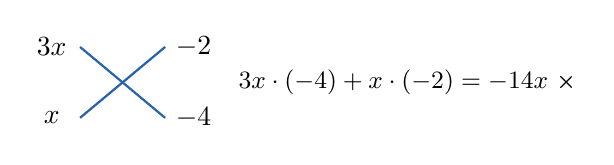
\begin{tikzpicture}[scale=0.9]
\node at (0, 0.5) {$3x$};
\node at (0, -0.5) {$x$};
\node at (2, 0.5) {$-2$};
\node at (2, -0.5) {$-4$};
\draw[thick, mainblue] (0.4, 0.5) -- (1.6, -0.5);
\draw[thick, mainblue] (0.4, -0.5) -- (1.6, 0.5);
\node[right, font=\small] at (2.5, 0) {$3x\cdot(-4)+x\cdot(-2)=-14x$ \texttimes};
\end{tikzpicture}
\end{center}
\begin{center}
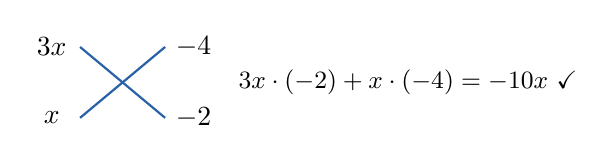
\begin{tikzpicture}[scale=0.9]
\node at (0, 0.5) {$3x$};
\node at (0, -0.5) {$x$};
\node at (2, 0.5) {$-4$};
\node at (2, -0.5) {$-2$};
\draw[thick, mainblue] (0.4, 0.5) -- (1.6, -0.5);
\draw[thick, mainblue] (0.4, -0.5) -- (1.6, 0.5);
\node[right, font=\small] at (2.5, 0) {$3x\cdot(-2)+x\cdot(-4)=-10x$ \checkmark};
\end{tikzpicture}
\end{center}
$\therefore\; 3x^2 - 10x + 8 = (3x-4)(x-2)$\\[8pt]
(2)\;$6x^2 + x - 2$\\
$a=6$ 的因数对：$1\times6,\; 2\times3$。$c=-2$ 的因数对：$1\times(-2),\; (-1)\times2$。\\[3pt]
\begin{center}
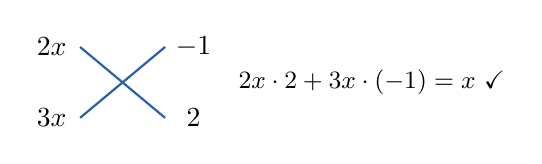
\begin{tikzpicture}[scale=0.9]
\node at (0, 0.5) {$2x$};
\node at (0, -0.5) {$3x$};
\node at (2, 0.5) {$-1$};
\node at (2, -0.5) {$2$};
\draw[thick, mainblue] (0.4, 0.5) -- (1.6, -0.5);
\draw[thick, mainblue] (0.4, -0.5) -- (1.6, 0.5);
\node[right, font=\small] at (2.5, 0) {$2x\cdot 2 + 3x\cdot(-1)=x$ \checkmark};
\end{tikzpicture}
\end{center}
$\therefore\; 6x^2 + x - 2 = (2x-1)(3x+2)$

% ──── 例题 4：分组分解 ────
\begin{examplebox}[【例题 4】分组分解法]
因式分解：\\[3pt]
(1)\;$x^3 - x^2 + x - 1$ \qquad (2)\;$a^2 - b^2 + 2a + 1$
\end{examplebox}

\textbf{解：}\\[3pt]
(1)\;$x^3 - x^2 + x - 1$\\
四项，两两分组：\\
$= (x^3 - x^2) + (x - 1)$\\
$= x^2(x - 1) + 1 \cdot (x - 1)$\\
$= (x - 1)(x^2 + 1)$\\[6pt]
(2)\;$a^2 - b^2 + 2a + 1$\\
重新组合：$(a^2 + 2a + 1) - b^2$\\
$= (a+1)^2 - b^2$\quad（前三项是完全平方，整体与 $b^2$ 构成平方差）\\
$= (a+1+b)(a+1-b)$\\
$= (a+b+1)(a-b+1)$

% ──── 例题 5：拆项添项 ────
\begin{examplebox}[【例题 5】拆项添项法]
因式分解：\\[3pt]
(1)\;$x^4 + 4$ \qquad (2)\;$x^3 - 7x + 6$
\end{examplebox}

\textbf{解：}\\[3pt]
(1)\;$x^4 + 4$（Sophie Germain 恒等式）\\
添上 $4x^2$ 再减去 $4x^2$：\\
$= x^4 + 4x^2 + 4 - 4x^2$\\
$= (x^2 + 2)^2 - (2x)^2$\quad（平方差）\\
$= (x^2 + 2 + 2x)(x^2 + 2 - 2x)$\\
$= (x^2 + 2x + 2)(x^2 - 2x + 2)$\\[6pt]
(2)\;$x^3 - 7x + 6$\\
尝试代入 $x=1$：$1 - 7 + 6 = 0$，所以 $(x-1)$ 是一个因式。\\[3pt]
拆 $-7x$ 为 $-x - 6x$：\\
$= x^3 - x - 6x + 6$\\
$= x(x^2-1) - 6(x-1)$\\
$= x(x+1)(x-1) - 6(x-1)$\\
$= (x-1)\big[x(x+1) - 6\big]$\\
$= (x-1)(x^2+x-6)$\\
$= (x-1)(x+3)(x-2)$

\begin{tipbox}[技巧：试根法辅助拆项]
对于三次多项式 $f(x)$，尝试 $f(1), f(-1), f(2), f(-2)$ 等简单值。\\
若 $f(a)=0$，则 $(x-a)$ 是一个因式，有助于确定拆项方向。
\end{tipbox}

% ──── 例题 6：配方 ────
\begin{examplebox}[【例题 6】配方法求最值]
(1)\quad 用配方法分解：$2x^2 - 12x + 10$。\\[3pt]
(2)\quad 用配方法求 $f(x) = x^2 - 4x + 7$ 的最小值。
\end{examplebox}

\textbf{解：}\\[3pt]
(1)\;$2x^2 - 12x + 10$\\
$= 2(x^2 - 6x) + 10$\\
$= 2(x^2 - 6x + 9 - 9) + 10$\\
$= 2(x-3)^2 - 18 + 10$\\
$= 2(x-3)^2 - 8$\\
$= 2\big[(x-3)^2 - 4\big]$\\
$= 2(x-3+2)(x-3-2)$\\
$= 2(x-1)(x-5)$\\[6pt]
(2)\;$f(x) = x^2 - 4x + 7 = (x^2-4x+4) + 3 = (x-2)^2 + 3$。\\
因为 $(x-2)^2 \geqslant 0$，所以 $f(x) \geqslant 3$。\\
当 $x=2$ 时取等号，$f(x)$ 的\textbf{最小值为 $3$}。

% ──── 例题 7：裂项求和 ────
\begin{examplebox}[【例题 7】裂项求和]
计算：$\displaystyle S = \frac{1}{1\times2} + \frac{1}{2\times3} + \frac{1}{3\times4} + \cdots + \frac{1}{99\times100}$。
\end{examplebox}

\textbf{解：}\\[3pt]
利用裂项公式 $\dfrac{1}{n(n+1)} = \dfrac{1}{n} - \dfrac{1}{n+1}$：\\[6pt]
$S = \left(\dfrac{1}{1} - \dfrac{1}{2}\right) + \left(\dfrac{1}{2} - \dfrac{1}{3}\right) + \left(\dfrac{1}{3} - \dfrac{1}{4}\right) + \cdots + \left(\dfrac{1}{99} - \dfrac{1}{100}\right)$\\[8pt]
相邻项\textbf{首尾相消}：\\
$= \dfrac{1}{1} - \dfrac{1}{100} = 1 - 0.01 = \boxed{\dfrac{99}{100}}$

\begin{tipbox}[裂项求和的关键]
找到裂项公式后，写出前几项和后几项，看清哪些项会消掉，哪些项会留下来。\\
最终结果 = \textbf{第一项的首部} $-$ \textbf{最后一项的尾部}。
\end{tipbox}

% ──── 例题 8：整体代换求值 ────
\begin{examplebox}[【例题 8】整体代换求值]
(1)\quad 已知 $a + b = 5$，$ab = 6$，求 $a^2 + b^2$ 和 $a^3 + b^3$ 的值。\\[3pt]
(2)\quad 已知 $x - \dfrac{1}{x} = 3$，求 $x^2 + \dfrac{1}{x^2}$ 的值。
\end{examplebox}

\textbf{解：}\\[3pt]
(1)\quad 由 $(a+b)^2 = a^2 + 2ab + b^2$，得\\
$a^2 + b^2 = (a+b)^2 - 2ab = 25 - 12 = \boxed{13}$。\\[6pt]
由立方和公式 $a^3+b^3 = (a+b)(a^2-ab+b^2)$，得\\
$a^3+b^3 = (a+b)\big[(a^2+b^2)-ab\big] = 5 \times (13-6) = 5\times7 = \boxed{35}$。\\[8pt]
(2)\quad $\left(x - \dfrac{1}{x}\right)^2 = x^2 - 2 + \dfrac{1}{x^2}$，\\
所以 $x^2 + \dfrac{1}{x^2} = \left(x - \dfrac{1}{x}\right)^2 + 2 = 9 + 2 = \boxed{11}$。

\begin{tipbox}[整体代换的常用恒等式]
已知 $a+b$ 和 $ab$，常用以下关系：\\
$a^2+b^2 = (a+b)^2-2ab$；\quad $a^2+b^2 = (a-b)^2+2ab$；\\
$a^3+b^3 = (a+b)^3-3ab(a+b)$；\quad $(a-b)^2 = (a+b)^2-4ab$。
\end{tipbox}

% ──── 例题 9：综合运算 ────
\begin{examplebox}[【例题 9】综合运算——化简求值]
先化简，再求值：$\left(\dfrac{x^2-4}{x^2-4x+4} + \dfrac{2-x}{x+2}\right) \div \dfrac{x}{x-2}$，其中 $x = \sqrt{3} + 2$。
\end{examplebox}

\textbf{解：}\\[3pt]
先化简各部分：\\
$\dfrac{x^2-4}{x^2-4x+4} = \dfrac{(x+2)(x-2)}{(x-2)^2} = \dfrac{x+2}{x-2}$\quad（$x \neq 2$）\\[6pt]
$\dfrac{2-x}{x+2} = \dfrac{-(x-2)}{x+2}$\\[6pt]
所以括号内：\\
$\dfrac{x+2}{x-2} + \dfrac{-(x-2)}{x+2} = \dfrac{(x+2)^2 - (x-2)^2}{(x-2)(x+2)}$\\[4pt]
分子：$(x+2)^2-(x-2)^2 = \big[(x+2)+(x-2)\big]\big[(x+2)-(x-2)\big] = 2x \cdot 4 = 8x$\\[4pt]
括号内 $= \dfrac{8x}{(x-2)(x+2)} = \dfrac{8x}{x^2-4}$\\[6pt]
除以 $\dfrac{x}{x-2}$ 即乘以 $\dfrac{x-2}{x}$：\\
$\dfrac{8x}{x^2-4} \cdot \dfrac{x-2}{x} = \dfrac{8x \cdot (x-2)}{(x+2)(x-2) \cdot x} = \dfrac{8}{x+2}$\\[6pt]
代入 $x = \sqrt{3}+2$：\\
$\dfrac{8}{\sqrt{3}+2+2} = \dfrac{8}{\sqrt{3}+4} = \dfrac{8(4-\sqrt{3})}{(4+\sqrt{3})(4-\sqrt{3})} = \dfrac{8(4-\sqrt{3})}{16-3} = \dfrac{8(4-\sqrt{3})}{13}$\\[4pt]
$= \boxed{\dfrac{32-8\sqrt{3}}{13}}$


% ==============================================================
% 第三部分：应用题
% ==============================================================
\section*{\textcolor{apppurple}{三、应用题}}

\begin{appbox}[【应用 1】几何中的因式分解]
一个正方形的边长增加 $3$ cm 后，面积增加了 $39$ cm$^2$。求原正方形的边长。
\end{appbox}

\textbf{解：}\\[3pt]
设原正方形边长为 $a$ cm。\\
新面积 $-$ 原面积 $= (a+3)^2 - a^2 = 39$。\\[3pt]
利用平方差公式：$(a+3)^2 - a^2 = (a+3+a)(a+3-a) = (2a+3) \cdot 3 = 3(2a+3)$。\\[3pt]
$3(2a+3) = 39 \implies 2a+3 = 13 \implies a = 5$。\\[3pt]
原正方形的边长为 $\boxed{5}$ cm。

\begin{appbox}[【应用 2】裂项求和在实际问题中的应用]
一根绳子长 $1$ 米。第一次剪去全长的 $\dfrac{1}{1\times2}$，第二次剪去剩余部分的 $\dfrac{1}{2\times3}$，第三次剪去剩余部分的 $\dfrac{1}{3\times4}$，以此类推，第 $n$ 次剪去剩余部分的 $\dfrac{1}{n(n+1)}$。\\
问：经过 $99$ 次后，绳子还剩多长？
\end{appbox}

\textbf{解：}\\[3pt]
每次剪去的是"剩余部分"的 $\dfrac{1}{k(k+1)}$，即每次\textbf{剩下}剩余部分的 $1-\dfrac{1}{k(k+1)}=\dfrac{k(k+1)-1}{k(k+1)}$。\\[4pt]
但这里题目更简单的理解是：\\
第 $k$ 次剪去的\textbf{绝对长度}为 $\dfrac{1}{k(k+1)}$ 米（即总量的 $\dfrac{1}{k(k+1)}$）。\\[3pt]
总剪去量 $= \displaystyle\sum_{k=1}^{99}\frac{1}{k(k+1)} = \sum_{k=1}^{99}\left(\frac{1}{k}-\frac{1}{k+1}\right) = 1 - \frac{1}{100} = \frac{99}{100}$。\\[3pt]
剩余长度 $= 1 - \dfrac{99}{100} = \boxed{\dfrac{1}{100}}$ 米。

\begin{appbox}[【应用 3】利用整式运算解决面积问题]
一块长方形土地，长比宽多 $4$ 米。若长和宽各增加 $3$ 米，面积就变为原来的 $2$ 倍。求原来长方形的长和宽。
\end{appbox}

\textbf{解：}\\[3pt]
设原来宽为 $x$ 米，则长为 $(x+4)$ 米。\\[3pt]
原面积 $= x(x+4)$；\quad 新面积 $= (x+3)(x+7)$。\\[3pt]
由题意：$(x+3)(x+7) = 2x(x+4)$。\\[3pt]
展开：$x^2 + 10x + 21 = 2x^2 + 8x$。\\[3pt]
整理：$x^2 - 2x - 21 = 0$。\\[3pt]
用十字相乘（或求根公式）：$x^2-2x-21$，判别式 $\Delta = 4+84 = 88$，\\
$x = \dfrac{2 \pm \sqrt{88}}{2} = 1 \pm \sqrt{22}$。\\[3pt]
因为 $x > 0$，所以 $x = 1 + \sqrt{22}$ 米（约 $5.69$ 米），\\
长 $= x + 4 = 5 + \sqrt{22}$ 米（约 $9.69$ 米）。\\[3pt]
$\boxed{\text{原来宽为 } (1+\sqrt{22}) \text{ 米，长为 } (5+\sqrt{22}) \text{ 米。}}$


% ==============================================================
% 第四部分：课堂练习
% ==============================================================
\section*{\textcolor{tipgreen}{四、课堂练习}}

\begin{enumerate}[leftmargin=18pt, label=\textbf{\arabic*.}, itemsep=8pt]
\item 因式分解：$2x^2 - 8$

\item 因式分解：$x^2 - 6x + 9$

\item 用十字相乘法分解：$x^2 + 3x - 28$

\item 用十字相乘法分解：$2x^2 - 5x - 3$

\item 分组分解：$xy - 2y + x - 2$

\item 拆项法分解：$x^3 + 2x^2 - 5x - 6$\\
{\small（提示：尝试 $f(2), f(-1), f(-3)$ 等值）}

\item 裂项求和：$\dfrac{1}{2\times4} + \dfrac{1}{4\times6} + \dfrac{1}{6\times8} + \cdots + \dfrac{1}{18\times20}$

\item 已知 $a + \dfrac{1}{a} = 4$，求 $a^2 + \dfrac{1}{a^2}$ 的值。
\end{enumerate}

\vspace{10pt}
\begin{knowledgebox}[参考答案]
\begin{enumerate}[leftmargin=18pt, label=\textbf{\arabic*.}, itemsep=6pt]
\item $2x^2 - 8 = 2(x^2-4) = \boxed{2(x+2)(x-2)}$

\item $x^2 - 6x + 9 = (x-3)^2 = \boxed{(x-3)^2}$

\item $x^2 + 3x - 28$：找 $p+q=3,\; pq=-28$，得 $p=7,\; q=-4$。\\
$= \boxed{(x+7)(x-4)}$

\item $2x^2 - 5x - 3$：十字相乘 $(2x+1)(x-3)$。\\
验证：$2x\cdot(-3)+1\cdot x = -5x$ \checkmark。\quad $= \boxed{(2x+1)(x-3)}$

\item $xy - 2y + x - 2 = y(x-2) + 1\cdot(x-2) = \boxed{(x-2)(y+1)}$

\item $f(2) = 8+8-10-6 = 0$，所以 $(x-2)$ 是因式。\\
$x^3+2x^2-5x-6 = x^3-2x^2+4x^2-8x+3x-6$\\
$= x^2(x-2)+4x(x-2)+3(x-2) = (x-2)(x^2+4x+3) = \boxed{(x-2)(x+1)(x+3)}$

\item $\dfrac{1}{k(k+2)} = \dfrac{1}{2}\!\left(\dfrac{1}{k}-\dfrac{1}{k+2}\right)$，其中 $k=2,4,6,\ldots,18$。\\
原式 $= \dfrac{1}{2}\left[\left(\dfrac{1}{2}-\dfrac{1}{4}\right)+\left(\dfrac{1}{4}-\dfrac{1}{6}\right)+\cdots+\left(\dfrac{1}{18}-\dfrac{1}{20}\right)\right]$\\
$= \dfrac{1}{2}\left(\dfrac{1}{2} - \dfrac{1}{20}\right) = \dfrac{1}{2} \cdot \dfrac{9}{20} = \boxed{\dfrac{9}{40}}$

\item $\left(a+\dfrac{1}{a}\right)^2 = a^2 + 2 + \dfrac{1}{a^2}$，所以 $a^2+\dfrac{1}{a^2} = 4^2 - 2 = \boxed{14}$
\end{enumerate}
\end{knowledgebox}

\vfill
\begin{center}
\small\textcolor{gray}{本讲义仅供教学参考，例题可根据学生水平调整难度。}
\end{center}

\end{document}
